\subsection{Automated Mask Generation}
\subsubsection{Introduction}
Detector masking is an important part of any x-ray scattering workflow as dead/hot pixels, streak errors, and beamstop associated features can be averaged into the data changing the signal and its statistical significance.
While some features, like the beamstop holder, can be easily observed and masked by hand other are much more difficult to observe even on large computer monitors.
Additionally, while dead/hot pixels and streaks are usually static the hot pixels associated with textured or single crystal scattering or cosmic rays are not.
Thus, coming up with an automated method for finding such erroneous pixels is important, especially as high flux diffraction beamlines can generate data very quickly.

While this problem can be quite complex in the most general case, we can use the annular symmetry of the powder scattering pattern to our advantage, by comparing a pixel against pixels in the same ring.
Since non-textured powder scattering should produce the same pixel intensity for a given ring we can mask any pixels which are $\alpha$ standard deviations away from the mean.
This method relies on the aforementioned pixel binning algorithm, as using miss sized bins will cause some pixels which should be in separate rings to be put together, and others which should be in the same ring to be separated.
In that case the masking algorithm will overestimate the number of pixels to be masked due to the additional statistical variation in the sample.

\subsubsection{Algorithm Design}
The masking algorithm procedure takes in the image and a description of the pixel positions in either distance from the point of incidence or in $Q$.
The image is then integrated twice, producing both the mean $I(Q)$ and the standard deviation of each $I(Q)$ ring.
The mask is created by comparing the pixel values against each ring's standard deviation and theshold $\alpha$.
Note that the theshold can be a funciton of distance from the point of incidence or $Q$.

\subsubsection{Test Cases}
To study the effectiveness of the masking we ran the algorithm against both simulated experimental data.
In the case of the simulated data four systems were created:
1) dead/hot pixels with varying numbers of defective pixels,
2) beamstop holder vith varying beamstop holder transmittance,
3) rotated beamstop holder vith varying beamstop holder transmittance,
and 4) beamstop holder with dead/hot pixels.
The base scattering was produced by
\begin{equation}
I = 100\cos(50r)^{2} + 150
\end{equation}
where $r$ is a pixel's distance from the beam point of incidence.
The positions of the dead/hot pixels were chosen at random as was the dead or hot nature of the defect. Dead pixels had values from 0 to 10, while hot pixels had values from 200 to 255.
The beamstop was positioned at the vertical center of the detector with an initial width of 60 pixels and final width of 120 pixels.
The hight of the beamstop was 1024 pixels.
The beamstop was calculated to attenuate the x-ray scattering signal at various transmittance, as various beamstop holder materials have different transmittance.
Two version of the masking algorithm were run for each test case, one using the standard even bin sizes for the integration step, and one where the bin sizes are tuned to the pixel $Q$ resolution as discussed in \ref{subsec:qres}.

\subsubsection{Results and Discussion}

\foreach \n in {100, 300, 500, 1000}{
\begin{figure}
  \centering
  \foreach \m in {masked}{
    \subfloat[]{\includegraphics[width=.5\textwidth]{bad_bin_dead_pixel_\m_\n}}
    \subfloat[]{\includegraphics[width=.5\textwidth]{dead_pixel_\m_\n}}
    }
\caption{Generated dead/hot pixel masks for a detector with $\n$ bad pixels. a) the poorly binned mask and b) the properly binned mask}
  \label{fig:dead_pixel_\n}
\end{figure}
}

\foreach \n in {10, 30, 50, 90}{
\begin{figure}
  \foreach \m in {raw, masked, missed}{
    \subfloat[]{\includegraphics[width=.3\textwidth]{\m_\n}}
    }
  \caption{Generated beamstop holder masks for a beamstop holder with $\n\%$ transmittance. a) the raw image, b) the masked image, c) and the missed pixels}
  \label{fig:bs_\n}
\end{figure}
}

\begin{figure}
        \foreach \m in {raw, masked, missed}{
        \subfloat[]{\includegraphics[width=.3\textwidth]{rotate_\m_50}
        }}
    \caption{Generated beamstop holder masks which is rotated away from verticle}
    \label{fig:rot_bs}
\end{figure}

\begin{figure}
    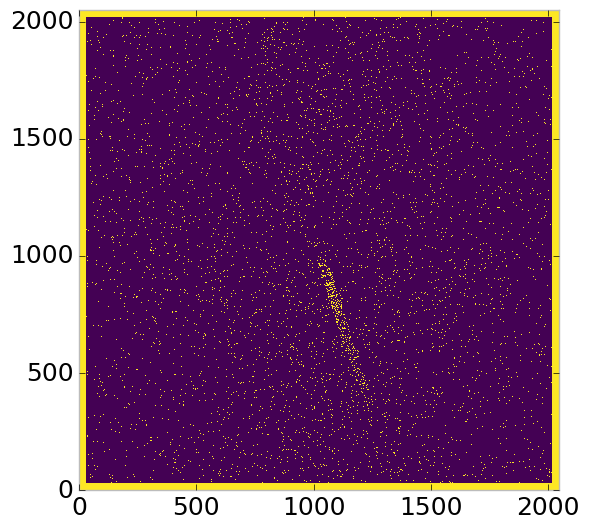
\includegraphics[width=\textwidth]{single_xtal_masked}
    \caption{Experimental data, with single crystal peaks}
    \label{fig:}
\end{figure}
%MAYBE ALSO ALSO NEED TO SHOW THE EFFECT OF CHANGING ALPHA FOR THE MASKING

ALSO ALSO ALSO SHOW SOME MASKS OF REAL DATA, INCLUDING DATA WITH SINGLE CRYSTAL/TEXTURE

Figures \ref{fig:dead_pixel_100}-\ref{fig:bs_90} show the results of the masking algorithm on simulated images.
The dead/hot pixel masking shows the importance of using the $Q$ resolution based bin sizes as the even bin based mask have a tendency to over mask the image, removing pixels which contain valuble signal.
This overmasking is caused by pixels being imporperly assocaited with one another by the even bins.
Figure \ref{fig:dead_pixel_100} indicates that the masking algorithm, with the proper binning, masks the image perfectly, with no missed bad pixels or good pixels masked.
This is not the case in figures \ref{fig:dead_pixel_300} - \ref{fig:dead_pixel_1000} as we can see pixels which should have been masked but were not.
Despite these missed pixels no pixles were imporperly masked in any of the well binned images.
These test cases are actually more difficult than experimental data, as the dynamic range of most detector causes the dead/hot pixels and single crystal/texture peaks to be orders of magnitude away from the desired signal.

The beamstop holder masks shown in figures \ref{fig:bs_10} - \ref{fig:bs_90}, which were all run with the $Q$ resolution binning show similar results across the transmitance range, missing only a small part of the beamstop holder near the point of incidence.
Near this point the beamstop holder becomes a statisticly signifigant part of the total number of pixels in a given ring, thus it can not be masked out using a statistical search of the rings.
For most PDF and XRD studies this small area can be masked automaticly by masking all the pixels who's distance from the point of incidence is smaller than a given radius $r$, or can be negelected outright as the area is not used in the analysis or refinement.
Similar results were produced for beamstop holders which were rotated away from the vericle position, as shown in figure \ref{fig:rot_bs}

\subsubsection{Conclusions}
In this section the masking algorithm, which relies on both $Q$ resolution based binning and a statistical approach to azimuthal symmetry, was developed.
The focus of this algorithm was to remove many unwanted detector features assocaited with pixel defect, beamstop holder associated scattering attenuation, and single crystal/texture peaks.
Simulated data was used to evaluate the beamstop holder and dead/hot pixel masking capacity, while experimental data was used to check for single crystal and texture based masking.
$Q$ resolution based binning was shown to be very important to avoid overmasking.
This masking algorithm is now in use in the data processing workflow and will be avaialable in scikit-beam soon.
